\begin{figure}[t]
\centering
% Vector drawing generated by tools/figures/snapshot.py; rerun it after changing the figure.
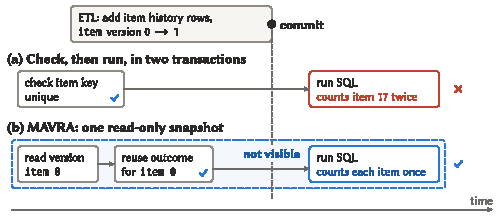
\includegraphics[width=\columnwidth]{figures/snapshot}%
\caption{\bt{Admission and snapshot binding (steps 4--6; L$n$: line $n$ of Algorithm~\ref{alg:snapshot-execution}). The ETL transaction bumps one of \code{item}'s 16 counter rows. Checks outside snapshots record verdicts only if the counters they read stay unchanged; a snapshot reuses verdicts at its own $v_s$.}{准入与快照绑定（步骤 4--6；L$n$ 指算法~\ref{alg:snapshot-execution} 第 $n$ 行）。ETL 事务给 \code{item} 的 16 行计数器之一加一。快照之外的检查仅在其读到的计数器前后不变时记录结论；快照只复用自身 $v_s$ 上的结论。}}
\label{fig:snapshot}
\Description{Top: Admission Admissible(q, R), tagged L2, with three requests drawn as call chips. run_metric ER@r1 is accepted (check): current, required filter kept, runs in s prime. run_sql ER@r0 is rejected (cross): r0 retired, current is r1. run_sql declaring none is rejected (cross): it drops i_is_current = 'Y', so item 17 would count twice. Middle, on a time axis: the ETL transaction (step 5) inserts history row (17, ..., 'N'); inside the same box, mavra_versions for item is drawn as 16 cells, one filled and marked +1; it commits at a point marked by a dashed vertical line. Snapshot s of Agent 2 (step 4) runs L5 item=0 and L7 hit before the commit line, then, past a label not visible, L11 counting item 17 once (check). Step 6, outside snapshots, after the commit: a counter read v=1, the check, another read v=1, equal, so the verdict is recorded. Snapshot s prime of Agent N (step 4) runs L5 item=1, L7 hit and L11 runs. Bottom: verdicts H_tx keyed by id(c) at v_s(dep(c)): KeyUnique(item.i_item_sk) at item=0, 1000/1000, pass, written by publication and reused by s; KeyUnique(item.i_item_sk) at item=1, 1001/1000, fail, written by maintenance; KeyUnique(item.i_item_sk, i_is_current='Y') at item=1, 1000/1000, pass, written by repair and reused by s prime. Versions are teal in the lanes and in the keys.}
\end{figure}
